\documentclass[12pt]{article}
\title{Comparison of Convolutional Neural Networks for Remote Sensing}
\date{2018-05-09}
\author{James Hurt}
\usepackage[margin=1.0in]{geometry}
\usepackage{graphicx}
\usepackage{subcaption}
\usepackage{cleveref}
\usepackage{indentfirst}
\usepackage{amsmath}
\usepackage{siunitx} % Required for alignment

\begin{document}
	\pagenumbering{arabic}
	
	%%%%%%%%%%%%%%%%
	% Title 
	%%%%%%%%%%%%%%%%
	\begin{flushright}
		James Hurt\break
		CS 8780\break
		9 May 2018
	\end{flushright}
	\begin{center}
		\huge{Comparison of Convolutional Neural Networks for Remote Sensing}
	\end{center}
	
	%%%%%%%%%%%%%%%%%%%%%%%
	% Technical Description
	%%%%%%%%%%%%%%%%%%%%%%%

	\begin{figure}[b!]
			\centering
			\begin{subfigure}[b]{0.3\linewidth}
				\centering
				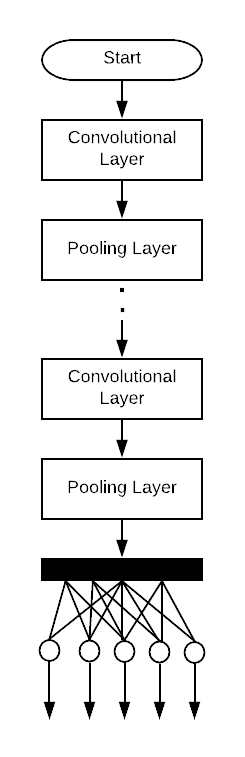
\includegraphics[scale=0.38]{img/custom_arc.png}
				\caption{Custom Shallow CNN}
				\label{fig:shallow_cnn}
			\end{subfigure}
			\begin{subfigure}[b]{0.3\linewidth}
				\centering
				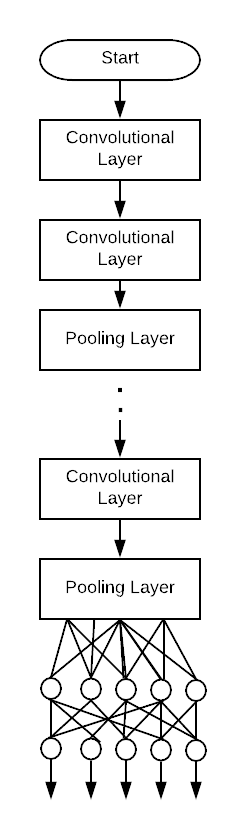
\includegraphics[scale=0.34]{img/vgg.png}
				\caption{VGG19}
			    \label{fig:deep_cnn}
			\end{subfigure}
			\begin{subfigure}[b]{0.3\linewidth}
				\centering
				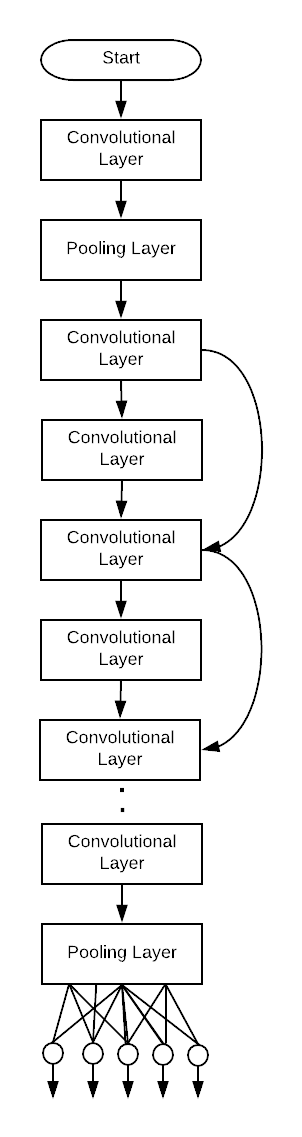
\includegraphics[scale=0.25]{img/res50.png}
				\caption{ResNet-50}
				\label{fig:deep_rnn}
			\end{subfigure}
			\caption{Architectures of the Compared CNN}
			\label{fig:architecture}
		\end{figure}

	\section{Technical Description}
	
Remote Sensing is a lucrative application for computational intelligence, with much of the recent research being in Convolutional Neural Networks. Within this discussion of neural networks for remote sensing, Deep Convolutional Neural Networks (DCNN) are the most popular. The popularity of convolutional neural networks can be attributed to the ability of a convolutional network to learn the features of the image, thus eliminating one of the greatest challenges in all of machine learning: feature selection and extraction. While CNN have proven very useful, one of the issues with DCNN is the high training time, even with GPU acceleration. In this project, I attempt to compare a shallow convolutional network with one of the first deep convolutional networks. I then take my comparison one step farther, by looking at the relative cost and benefit of residual neural networks. 
		
I chose to make my comparison of CNN for the application of Remote Sensing because I am very interested in Remote Sensing. I think the ability to detect object from satellite imagery has many applications in every day life and can better the lives of common people as well as aid industry in understanding what is around their facilities. 
		
		\subsection{Shallow Convolutional Neural Network}
		
The shallow convolutional neural network used in this project combines many techniques of fully connected networks previously used for pattern recognition. The architecture of the network can be see in \Cref{fig:shallow_cnn}.
		
The architecture of the network has a total of 12 layers. The first 10 layers are alternating 2D Convolutional layers layers with a 3x3 kernel size and 2D Max Pooling layers with a 2x2 Pooling Window. After these 10 layers, feature extraction is finished, and a flattening layer is introduced to put the data into a single vector for the final fully connected softmax layer. 
		
		
		\subsection{Deep Convolutional Neural Network}
		
The Deep Convolutional Neural Network used for comparison in this project is VGG 19 \cite{vgg}. The VGG 19 network, as the name suggests, has 19 total layers. This count, however, does not include the pooling layers. The basic architecture can been seen in \Cref{fig:deep_cnn}. 

VGG19 has 16 convolutional layers and 4 pooling layers. The interesting quality about VGG19 is that the final pooling layer does not connect directly to the softmax output layer. Instead, the final pooling layer is a 3-layer multilayer perceptron (MLP) \cite{ci_book} The final layer of this MLP is a softmax layer for classification. 

		\subsection{Deep Residual Convolutional Neural Network}

The final neural network used for comparison in this project is a Deep Residual Convolutional Neural Network (DRNN). I chose to use ResNet-50 \cite{resnet50}, a standard DRNN for comparison developed by Microsoft Research. The architecture of this network can be seen in \Cref{fig:deep_rnn}.

ResNet-50 begins with a single convolutional layer, followed by a single pooling layer, followed by 49 convolutional layers that are residual, meaning that there is a connection from layer \textit{N} to both layer \textit{N+1} as well as layer \textit{N+2}. This connection exists so that the error from the two connections to the \textit{N+2} layer can be summed when performing backpropagation, thus slowing the disappearance of the gradient. The disappearing gradient is one of the greatest challenges of using the gradient descent method. 
	
	\section{Algorithm Design}
	
	\begin{figure}[t!]
		\centering
		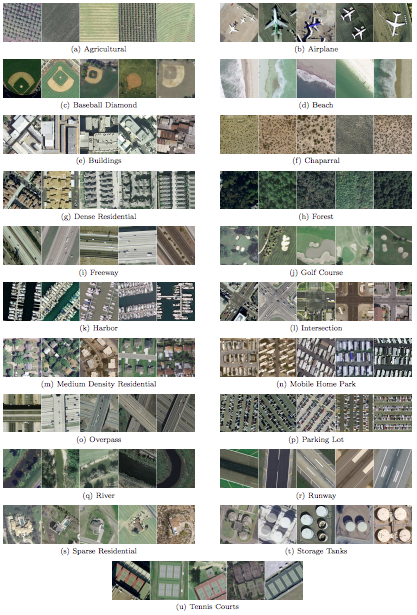
\includegraphics[width=0.5\linewidth]{img/ucm.png}
		\caption{UCMerced Dataset with 21 classes}
		\label{fig:ucm}
	\end{figure}
	
	\subsection{Dataset Selection}
The algorithm I designed for comparing these various CNN involved 2 datasets: a 3 class dataset and the benchmark UC Merced Dataset \cite{ucm}. The 3 class problem is a subset of the UCMerced dataset. I chose 3 classes from the UCMerced dataset: agricultural, airplane, and baseball diamond. While the test dataset is small, the UCMerced dataset, seen in \Cref{fig:ucm} is not. It has 21 classes, each with 100 images each. This dataset is not the largest available as far as benchmark Remote Sensing is concerned, but I felt it was a good representative for my comparison, because I didn't want too challenging a dataset. 

I chose to use 2 datasets because I felt that using only one would not give me enough of a picture to draw conclusions. Perhaps, if I had chosen just one dataset, the dataset I picked was particularly suited to one of these methods, but if I chose 2, then I would have enough to draw somewhat of a conclusion. Certainly, only 2 datasets is not enough for a generalization, but it does allow me to eliminate the possibility of choosing a biased dataset.

I also chose to have a small and large dataset, because there are many instances of binary classification needed in everyday life, so looking at a 3 class problem as well as a large, 21 class problem, would allow me to see if one method was better for large but not small or vice versa. If I found that the shallow could better handle the 3 class problem or maybe if the shallow CNN was within 1\% cross validation accuracy, for example, then I could say that binary classifiers could settle for a shallow CNN, thus relieving the long training times required for Deep CNN or RNN. 

	\subsection{Parameter Selection}
After choosing the datasets to use, I had to decide on the parameters for the algorithms. The choices I had to make specifically were the loss function and the optimizer. I needed to choose one of each that would be used in all 3 algorithms. I had to use the same one to ensure a fair comparison. 

The loss function I decided to use was \textbf{categorical crossentropy} \cite{cross_entropy}: 
		
\[
		H(q,p) =  \int q(x) log(q(x) / p(x)) \mathrm{d}x
\]

Crossentropy, as discussed in the first Computational Intelligence class, is a useful loss function because it harshly punishes output that is very far from the correct value. It is more punishing than standard error and can help a network converge in less epochs. 

For the optimizer, I started with knowledge of gradient descent from the previous Computational Intelligence class, and decided to choose a similar optimizer for my CNN, \textbf{Stochastic Gradient Descent (SGD)} \cite{sgd}:

\[
	w(t+1) = w(t) - \eta \frac{\partial}{\partial w} \ell(f(x_t), y_t)
\]

The function of SGD is very similar to gradient descent in that we are attempting to move the opposite direction of the error function in search of a set of parameters such that there exists a global minimum for error.

	\subsection{Comparison Algorithm}
	
To compare the three algorithms, I designed two separate Python classes to utilize the Tensorflow GPU and Keras libraries for Deep Learning. The first class was for the shallow CNN. I manually defined the 12 layers for the model, as well as built general utility functions to take in a directory of images and generate the 5 folds and to take in a list of filenames and generate an array of 3D matrices that were the numerical representations of the images required by Keras for training the networks. After defining these functions, I build logic to run a cross validation experiment. on the given images and storing results in a variable for later use.

Once I had the shallow network build and working, I built another class for the 2 deep networks: VGG19 and ResNet-50. This class utilized many of the functions I wrote for the shallow network. The main difference was the model. For the shallow, I had to build the model from scratch. For these networks, I was able to import the convolutional and pooling layers from Keras. I only had to build the final layer for classification with a softmax activation function and attach it to the end of the final convolutional layer. I only needed 1 class for both networks because I could pass a boolean to the class to tell it whether to import ResNet-50 or VGG19. This class also had logic to perform a cross validation experiment with 1 function call and store results for later analysis. 

After I had the ability to perform cross validation experiments with 1 function call, I built a script to bring in the two datasets, train them for 10, 20, 30, 40, and 50 epochs, and record the performance of all 3 nets on both networks for the 5 different lengths of training. One of the concerns of this project was the training time, so I feel it is important to note that all experiments were GPU accelerated with 4 Nvidia GPUs using cuDNN, a C++ CUDA library for Deep Learning on Nvidia GPUs, which was then tied into Tensorflow-GPU, which is optimized for cuDNN. 
	
	\section{Experiment Results}
	
	The experiments run were 5-fold cross validation on  both the test dataset and UCMerced for 10, 20, 30, 40, and 50 epochs on the ShallowCNN, Deep CNN (VGG19), and Deep RNN (ResNet-50)
	\subsection{Test Dataset}

	\begin{table}[h!]
		\begin{center}
			\caption{Average Cross Validation Accuracy for Test Dataset}
			\label{table:test}
			\begin{tabular}{l | S | S | S | S |  S}
				\textbf{Method} & \textbf{10 Epochs} & \textbf{20 Epochs} & \textbf{30 Epochs} & \textbf{40 Epochs} & \textbf{50 Epochs} \\
				\hline
				Shallow CNN & 91.2\% & 92.5\% & 92.2\% & 89.7\% & 92.8\% \\
				Deep CNN & 35.1\% & 33.1\% & 33.1\% & 57.7\% & 33.5\% \\
				Deep RNN & 75.5\% & 94.5\% & 92.3\% & 97.3\% & 94.9\% \\
				
			
			\end{tabular}					
		
		
		\end{center}
	
	\end{table}
	\subsection{UCMerced Dataset}
	\begin{table}[h!]
		\begin{center}
			\caption{Average Cross Validation Accuracy for UCMerced Dataset}
			\label{table:ucm}
			\begin{tabular}{l | S | S | S | S |  S}
				\textbf{Method} & \textbf{10 Epochs} & \textbf{20 Epochs} & \textbf{30 Epochs} & \textbf{40 Epochs} & \textbf{50 Epochs} \\
				\hline
				Shallow CNN & 38.9\% & 38.6\% & 35.3\% & 26.6\% & 33.2\% \\
				Deep CNN & 17.9\% & 15.1\% & 18.6\% & 4.9\% & 53.1\% \\
				Deep RNN & 94.8\% & 96.2\% & 96.2\% & 96.4\% & 97.8\% \\
				
			
			\end{tabular}					
		
		
		\end{center}
	
	\end{table}
	
	\section{Analysis}
	
	\section{Code}
	
	The code for this project can be seen in the \textbf{Code} folder. 
	
	
%%%%%%%%%%%%%%%%
%		 REFERENCES
%%%%%%%%%%%%%%%%%
	\newpage
	\bibliography{bibliography} 
	\bibliographystyle{ieeetr}




\end{document}